\section{Proposed Taxonomy}
\begin{itemize}
	\item Looked at it from perspective of architecture
	\item Attacks
		\begin{itemize}
			\item First Split on Architecture Legal, reason: bug needing bugfix or not
			\item If illegal, split on fault type, reason: obvious
			\item If pagefault, further split on page permission bit, reason: obvious
			\item If legal, split on hardware buffer affected, reason: the module that needs to be rethought
		\end{itemize}

	\item Defenses
		\begin{itemize}
			\item defenses were catergorized based on implementation where, how much, when, etc
			\item First split on where is defense implemented, reason: determine what you can implement new hardware vs new compiler
			\item Firmware - microcode changes, pick and choose if it applies
			\item Software further split on OS or App, reason: Do you have control over OS, can you control OS, do you trust OS, answer no to any look at App level fixes
			\item Hardware futher split on change to existing hardware or completely new concept, reason: implementation cost
		\end{itemize}

\end{itemize}

\begin{center}
\begin{figure}[!p]
    \makebox[\textwidth]{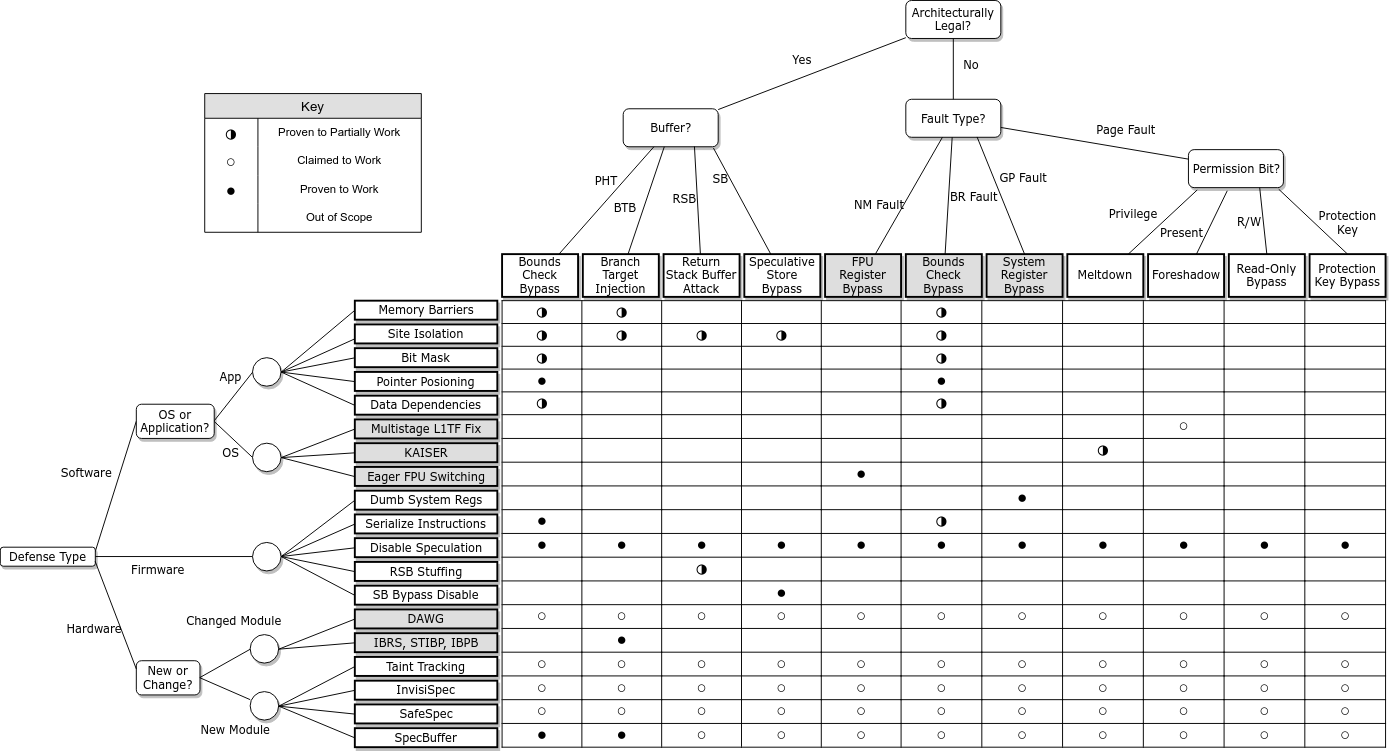
\includegraphics[width=1.1\paperwidth,angle=270]{categorization}}
    %\captionsetup{justification=centering}
    \caption{Full taxonomy of different attacks and defenses and what they cover}
    \label{fig:categorization}
\end{figure}
\afterpage{\clearpage}
\end{center}
